\let\negmedspace\undefined
\let\negthickspace\undefined
\documentclass[journal]{IEEEtran}
\usepackage[a5paper, margin=10mm, onecolumn]{geometry}
%\usepackage{lmodern} % Ensure lmodern is loaded for pdflatex
\usepackage{tfrupee} % Include tfrupee package

\setlength{\headheight}{1cm} % Set the height of the header box
\setlength{\headsep}{0mm}     % Set the distance between the header box and the top of the text
\usepackage{gvv-book}
\usepackage{gvv}
\usepackage{cite}
\usepackage{amsmath,amssymb,amsfonts,amsthm}
\usepackage{algorithmic}
\usepackage{graphicx}
\usepackage{textcomp}
\usepackage{xcolor}
\usepackage{txfonts}
\usepackage{listings}
\usepackage{enumitem}
\usepackage{mathtools}
\usepackage{gensymb}
\usepackage{comment}
\usepackage[breaklinks=true]{hyperref}
\usepackage{tkz-euclide} 
\usepackage{listings}
% \usepackage{gvv}                                        
\def\inputGnumericTable{}                                 
\usepackage[latin1]{inputenc}                                
\usepackage{color}                                            
\usepackage{array}                                            
\usepackage{longtable}                                       
\usepackage{calc}                                             
\usepackage{multirow}                                         
\usepackage{hhline}                                           
\usepackage{ifthen}                                           
\usepackage{lscape}
\usepackage{circuitikz}
\usepackage{float}
\renewcommand{\thefigure}{\theenumi}
\renewcommand{\thetable}{\theenumi}
\setlength{\intextsep}{10pt} % Space between text and floats


\numberwithin{equation}{enumi}
\numberwithin{figure}{enumi}
\renewcommand{\thetable}{\theenumi}




% Marks the beginning of the document
\begin{document}
\bibliographystyle{IEEEtran}
\vspace{3cm}

\title{CE\\2012}
\author{EE24BTECH11063 - Y.Harsha Vardhan Reddy}
\maketitle

\bigskip

\renewcommand{\thefigure}{\theenumi}
\renewcommand{\thetable}{\theenumi}

\section*{Q.1-Q.25 carry one mark each}
\begin{enumerate}

\item  A smooth rigid retaining wall moves as shown$\ref{fig:1}$ in the sketch causing the backfill material to fail. The backfill material is homogeneous and isotropic, and obeys the Mohr-Coulomb failure criterion. The major principal stress is
\begin{figure}[H]
    \centering
    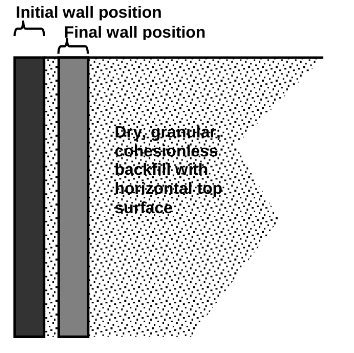
\includegraphics[scale=0.5]{figs/1.png} % Change 0.5 to any scale factor
    \caption{}
    \label{fig:1}
\end{figure}
\begin{enumerate}
    \item parallel to the wall face and acting downwards
    \item normal to the wall face
    \item oblique to the wall face acting downwards
    \item oblique to the wall face acting upwards
\end{enumerate}

\item An embankment is to be constructed with a granular soil (bulk unit weight = 20 kN/m$^3$) on a saturated clayey silt deposit (undrained shear strength = 25 kPa). Assuming undrained general shear failure and bearing capacity factor of 5.7, the maximum height (in m) of the embankment at the point of failure is

\begin{enumerate}
\begin{multicols}{4}
    \item 7.1
    \item 5.0
    \item 4.5
    \item 2.5
    \end{multicols}
\end{enumerate}

\item A trapezoidal channel is 10.0 m wide at the base and has a side slope of 4 horizontal to 3 vertical. The bed slope is 0.002. The channel is lined with smooth concrete $\brak{\text{Manning's } n=0.012}$. The hydraulic radius $\brak{\text{in m}}$ for a depth of flow of 3.0 m is

\begin{enumerate}
\begin{multicols}{4}
    \item 20.0
    \item 3.5
    \item 3.0
    \item 2.1
    \end{multicols}
\end{enumerate}

\item A rectangular open channel of width 5.0 m is carrying a discharge of 100 m$^3$/s. The Froude number of the flow is 0.8. The depth of flow (in m) in the channel is

\begin{enumerate}
\begin{multicols}{4}
    \item 4
    \item 5
    \item 16
    \item 20
    \end{multicols}
\end{enumerate}
\item  The circular water pipes shown in the sketch$\ref{fig:2}$ are flowing full. The velocity of flow (in m/s) in the branch pipe "R" is
	\begin{figure}[H]
    
			\centering
			\scalebox{0.5}{
\begin{circuitikz}
\tikzstyle{every node}=[font=\normalsize]
\draw (4.25,10) to[short] (11,10);
\draw (4.25,7.75) to[short] (6.75,7.75);
\draw (8.5,7.75) to[short] (11,7.75);
\draw (6.75,5.25) to[short] (6.75,7.75);
\draw (8.5,5.25) to[short] (8.5,7.75);
\draw [dashed] (6,6.75) -- (9.25,6.75)node[pos=0.9,above, fill=white]{R};
\draw [->, >=Stealth] (7.5,7.25) -- (7.5,6)node[pos=0.85,below, fill=white]{V=?};
\draw [->, >=Stealth] (9.25,6) -- (8.5,6.5);
\draw [short] (9.25,6) -- (11,6)node[pos=1, fill=white]{dia = 2 m};
\draw [dashed] (10,7.25) -- (10,10.5)node[pos=0.95,right, fill=white]{Q};
\draw [dashed] (5,7.25) -- (5,10.5)node[pos=0.95,left, fill=white]{P};
\draw [->, >=Stealth] (3.75,9) -- (5.75,9)node[pos=0, fill=white]{V=6m/s};
\draw [->, >=Stealth] (8.75,9) -- (10.75,9)node[pos=0.95,right, fill=white]{V=5m/s};
\draw [->, >=Stealth] (6.25,10.5) -- (6,9.5);
\draw [->, >=Stealth] (8.75,10.5) -- (9,9.5);
\draw [short] (8.25,10.5) -- (8.75,10.5)node[pos=0,left, fill=white]{dia = 4m};
\draw (6.25,10.5) to[short] (6.75,10.5);
\end{circuitikz}
}

			\label{fig:2}
			\caption{}
		\end{figure}
\begin{enumerate}
\begin{multicols}{4}
    \item 3
    \item 4
    \item 5
    \item 6
    \end{multicols}
\end{enumerate}

\item The ratio of actual evapo-transpiration to potential evapo-transpiration is in the range

\begin{enumerate}
\begin{multicols}{4}
    \item 0.0 to 0.4
    \item 0.6 to 0.9
    \item 0.0 to 1.0
    \item 1.0 to 2.0
    \end{multicols}
\end{enumerate}

\item A sample of domestic sewage is digested with silver sulphate, sulphuric acid, potassium dichromate and mercuric sulphate in chemical oxygen demand (COD) test. The digested sample is then titrated with standard ferrous ammonium sulphate (FAS) to determine the un-reacted amount of

\begin{enumerate}
\begin{multicols}{2}
    \item mercuric sulphate
    \columnbreak
    \item potassium dichromate
    \end{multicols}
    \begin{multicols}{2}
    \item silver sulphate
    \item sulphuric acid
    \end{multicols}
\end{enumerate}

\item \textbf{Assertion [a]:} At a manhole, the crown of the outgoing sewer should not be higher than the crown of the incoming sewer. \\
\textbf{Reason [r]:}   Transition from a larger diameter incoming sewer to a smaller diameter outgoing sewer at a manhole should not be made. \\
The \textbf{CORRECT} option evaluating the above statements is:

\begin{enumerate}
    \item Both \textbf{[a]} and \textbf{[r]} are true and \textbf{[r]} is the correct reason for \textbf{[a]}
    \item Both \textbf{[a]} and \textbf{[r]} are true but \textbf{[r]} is not the correct reason for \textbf{[a]}
    \item Both \textbf{[a]} and \textbf{[r]} are false
    \item \textbf{[a]} is true but \textbf{[r]} is false
\end{enumerate}

\item Two major roads with two lanes each are crossing in an urban area to form an un-controlled intersection. The number of conflict points when both roads are two-way is X and when both roads are one-way is Y. The ratio of X to Y is

\begin{enumerate}
\begin{multicols}{4}
    \item 4
    \item 5
    \item 16
    \item 20
    \end{multicols}
\end{enumerate}

\item Two bitumen samples "X" and "Y" have softening points 45\degree C and 60\degree C, respectively. Consider the following statements:

\begin{enumerate}
    \item[I.] Viscosity of "X" will be higher than that of "Y" at the same temperature.
    \item[II.] Penetration value of "X" will be lesser than that of "Y" under standard conditions.
\end{enumerate}

The \textbf{CORRECT} option evaluating the above statements is

\begin{enumerate}
    \item Both I and II are TRUE
    \item I is FALSE and II is TRUE
    \item Both I and II are FALSE
    \item I is TRUE and II is FALSE
\end{enumerate}

\item  Road roughness is measured using

\begin{enumerate}
    \item Benkelman beam
    \item Bump integrator
    \item Dynamic cone penetrometer
    \item Falling weight deflectometer
\end{enumerate}

\item Which of the following errors can be eliminated by reciprocal measurements in differential leveling?\\
        \begin{enumerate}
            \item[I] Error due to earth's curvature
            \item[II] Error due to atmospheric refraction
        \end{enumerate}

\begin{enumerate}
    \begin{multicols}{4}
        \item Both I and II
        \item I only
        \item II only
        \item Neither I nor II
    \end{multicols}
\end{enumerate} 
\section{Q.26-Q.55 carry two marks each.}
\item The error in $\left. \frac{d}{dx} f(x) \right|_{x = x_0}$ for a continuous function estimated with $h = 0.03$ using the central difference formula
\[
\left. \frac{d}{dx} f(x) \right|_{x = x_0} \approx \frac{f(x_0 + h) - f(x_0 - h)}{2h},
\]
is $2 \times 10^{-3}$. The values of $x_0$ and $f(x_0)$ are 19.78 and 500.01, respectively. The corresponding error in the central difference estimate for $h = 0.02$ is approximately
\begin{enumerate}
    \begin{multicols}{4}
        \item $1.3 \times 10^{-4}$
        \item $3.0 \times 10^{-4}$
        \item $4.5 \times 10^{-4}$
        \item $9.0 \times 10^{-4}$
    \end{multicols}
\end{enumerate}
\end{enumerate}


\end{document}

